\chapter{Introducere}
% \chapter*{Introducere}
% \addcontentsline{toc}{chapter}{Introducere}

\section{Prezentarea generală a temei}
    \paragraph{} Containerizarea, sau virtualizarea la nivel de sistem de operare este o paradigmă a sistemului de operare în care \textit{kernelul} permite existența a mai multor instanțe izolate ale utilizatorului. Astfel de instanțe, numite containere (Solaris, Docker), zone (Solaris), servere private virtuale (OpenVZ), partiții, medii virtuale (VEs), \textit{kerneluri} virtuale (DragonFly BSD) sau închisori (FreeBSD jail sau chroot jail), pot părea ca niște computere reale din punctul de vedere al programelor care rulează în ele. Un program care rulează pe un sistem de operare obișnuit poate vedea toate resursele (dispozitive conectate, fișiere și foldere, \textit{network share}-uri, putere a procesorului, capacități hardware cuantificabile) ale acelui computer. Cu toate acestea, programele care rulează în interiorul unui container pot vedea doar conținutul și dispozitivele destinate containerului. \cite{wiki:osv}
    \paragraph{} Pe sistemele de operare similare Unix, această caracteristică poate fi văzută ca o implementare avansată a mecanismului standard \textit{chroot}, care schimbă folderul rădăcină aparent pentru procesul de rulare curent și copiii săi. În plus față de mecanismele de izolare, \textit{kernelul} oferă și funcții de gestionare a resurselor pentru a limita impactul activităților unui container asupra altor containere. \cite{wiki:osv}
    \paragraph{} Virtualizarea la nivel de sistem de operare este folosită în mod obișnuit în mediile de găzduire virtuale, unde este utilă pentru alocarea în siguranță a resurselor hardware finite între un număr mare de utilizatori. Administratorii de sistem o pot utiliza, de asemenea, pentru consolidarea hardware-ului unui server, prin mutarea serviciilor de pe gazde separate pe un singur server în containerele. \cite{wiki:osv}
        \begin{figure}[h!]
            \centering
            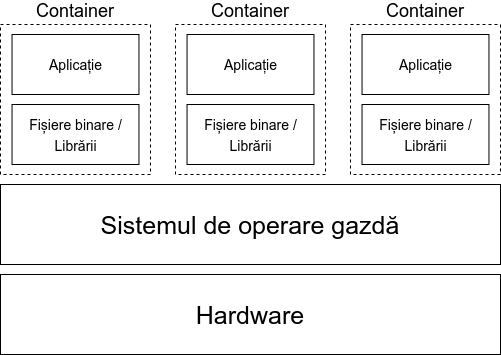
\includegraphics[width=0.75\textwidth]{virt}
            \caption{Virtualizarea la nivel de sistem de operare}
            \label{fig:virt}
        \end{figure}
    \paragraph{} Alte scenarii tipice includ separarea mai multor programe în mai multe containere pentru o securitate mai bună, independență hardware și funcții adiționale de gestionare a resurselor. Implementările de virtualizare la nivel de sistem de operare, capabile să migreze direct, pot fi de asemenea utilizate pentru echilibrarea dinamică a resurselor utilizate de containere între nodurile dintr-un cluster. \cite{wiki:osv}
    \paragraph{} De asemenea, acest tip de virtualizare este folosită în dezvoltarea de aplicații pentru rezolvarea problemelor de dependențe (lipsa acestora sau conflictele dintre ele) și a diferențelor dintre platforme. \cite{merkel2014docker}
        \begin{figure}[h!]
            \centering
            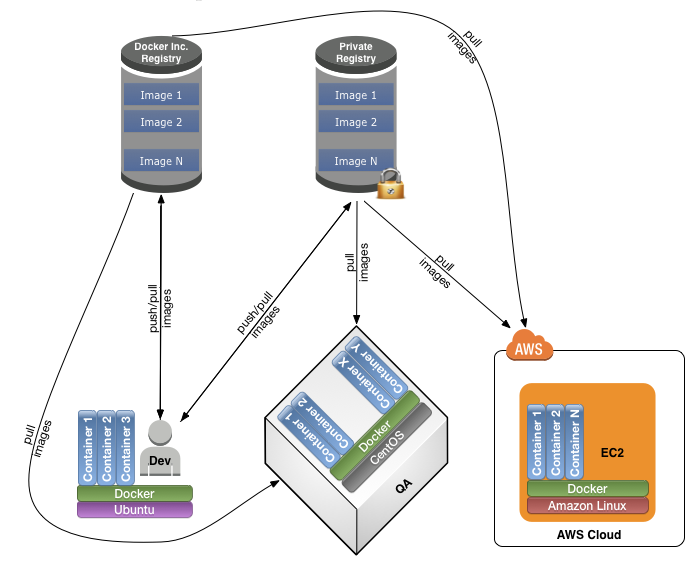
\includegraphics[width=1\textwidth]{workflow}
            \caption{Fluxul de lucru cu aplicația Docker \cite{merkel2014docker}}
            \label{fig:workflow}
        \end{figure}
    % TODO Mai adauga
    % TODO Utilizari?
    % \subsection{Tipul lucrării şi subdomeniul specific în care se încadrează tema}
    % \subsection{Prezentarea domeniului din care face parte tema aleasa (de exp aplicatie Android pentru...)}
    % \subsection{Câteva repere istorice relativ la temă şi rezultate cunoscute (starea actuală a domeniului eventual).}

\section{Scopul lucrării}
    \paragraph{} Scopul acestei lucrări este de a dezvolta o aplicație de virtualizare folosind funcțio\-nalitățile puse la dispoziție de către \textit{kernelul} Linux. Această aplicație urmănd ca exemple principale aplicația Docker și specificațiile OCI.

% TODO Structura lucrarii
% \section{Structura lucrării}
%     \subsection{O scurta prezentare a lucrarii, adica ce cuprinde fiecare capitol}
%     \subsection{Structura lucrării, cu descrierea succintă a fiecărui capitol,}

% TODO Contextul actual
% \section{Contextul actual}

\section{Soluții existente}
    \subsection{chroot}
        \paragraph{} \textbf{chroot} este un apel de sistem care schimbă directorul rădăcină aparent pentru procesul de rulare curent și pentru copiii săi. Acesta a fost introdus în cursul dezvoltării versiunii 7 Unix în 1979 și a fost adăugat la BSD de Bill Joy la 18 martie 1982. \cite{kamp2000jails}
        \paragraph{} Operația \textit{chroot} nu este destinată să se apere împotriva manipulării intenționate de către utilizatorii privilegiați (root). În majoritatea sistemelor, contextele \textit{chroot} nu sunt adăugate corect și programele \textit{chroot}-ate cu privilegii suficiente pot efectua un al doilea \textit{chroot} pentru a ieși din mediul respectiv. Pentru a atenua riscul acestei slăbiciuni în materie de securitate, programele trebuie să renunțe la privilegiile de administrator imediat după operația de \textit{chroot}, sau ar trebui utilizate în schimb alte mecanisme - cum ar fi închisorile FreeBSD. Unele sisteme, cum ar fi FreeBSD, iau măsuri de precauție pentru a preveni un al doilea atac \textit{chroot}. \cite{freebsd:chroot}

    \subsection{FreeBSD Jail}
        \paragraph{} \textbf{jail} este o implementare a virtualizării la nivel de sistem FreeBSD, care permite administratorilor de sistem să partiționeze un sistem FreeBSD în mai multe mini-sisteme independente numite închisori, toate care au același kernel. \cite{jail} Acesta este implementat printr-un apel de sistem, \textit{jail(2)}, precum și o utilitate de tip userland, \textit{jail(8)}. \cite{wiki:jail}

    \subsection{LXC}
        \paragraph{} \textbf{LXC} (Linux Containers) este o metodă de virtualizare la nivel de sistem de operare folosită pentru rularea mai multor sisteme Linux (containere) izolate pe o gazdă utilizând un singur \textit{kernel} Linux. \cite{wiki:lxc}
        \paragraph{} \textit{Kernelul} Linux oferă funcționalitatea cgroups care permite limitarea și prioritizarea resurselor (procesor, memorie, I/O, rețea etc.) fără a fi necesară pornirea unor mașini virtuale și, de asemenea, funcționalitatea de izolare a spațiului de nume care permite izolarea completă a unei aplicații vedere a mediului de operare. \cite{wiki:lxc}
        \paragraph{} LXC combină cgrupurile nucleului și suportul pentru spațiile de nume izolate pentru a oferi un mediu izolat pentru aplicații. Versiunile anterioare de Docker au folosit LXC ca driver de execuție a containerelor, deși LXC a devenit opțional în v0.9, iar suportul a fost oprit în Docker v1.10. \cite{lxc_docker}\cite{wiki:lxc}

    \subsection{docker}
        \paragraph{} \textbf{Docker} este un set produse de tipul \textit{platform as a service} (PaaS) care utilizează virtualizarea la nivel de sistem de operare pentru a livra software în pachete numite containere. Containerele sunt izolate unele de celelalte și conțin propriile programe, biblioteci și fișiere de configurare; ele pot comunica între ele prin canale bine definite. Toate containerele sunt administrate de un \textit{kernelul} sistemului de operare și, prin urmare, folosesc mai puține resurse decât mașinile virtuale. \cite{wiki:docker}

\section{Open Container Initiative (OCI)}
    \paragraph{} Inițiativa Open Container (OCI) este proiect realizat de către fundația Linux, cu scopul de a crea standarde în jurul formatelor de containere și în jurul rulării acestora. OCI a fost lansată pe 22 iunie 2015 de Docker, CoreOS și alți lideri din industria containerelor.
    \paragraph{} OCI conține în prezent două specificații: Specificația pentru rulare (runtime-spec) și Specificația pentru imagini (imagine-spec). Specificația pentru rulare prezintă modul de a rula un „pachet de sisteme de fișiere" (\textit{filesystem bundle}) care este despachetat pe disc. La un nivel înalt, o implementare OCI ar descărca o imagine OCI, apoi ar despacheta imaginea în sistemul de fișiere al unui \textit{runtime} OCI. Acest pachet urmează să fie rulat de către \textit{runtime}.
    \paragraph{} Formatul de imagine OCI conține suficiente informații pentru a lansa o aplicație pe o platforma țintă (de exemplu, comandă, argumente, variabile de mediu etc.). Această specificație definește modul de creare a unei imagini OCI, care va fi realizată în general de către un sistem de compilare, și de generare a unui \textit{image manifest}, a unei serializări de sistem de fișiere (\textit{layer}) și a unei configurații a imaginii. La un nivel înalt, \textit{image manifest}-ul conține metadate despre conținutul și dependențele imaginii. Configurația imaginii include informații, cum ar fi argumentele aplicației, medii, etc.

\section{Motivație}
    \paragraph{} Motivul pentru care am ales această temă este pentru a mă familiariza cu mecanismele care stau in spatele multor aplicații de virtualizare folosite în industrie și pentru a învăța un nou limbaj de programare. Am ales limbajul de programare rust datorită similarității acestuia cu limbajul C++ și datorită designului sau care pune accentul pe performanță și siguranță. \cite{jung2017rustbelt}